\documentclass[a4paper]{article}

\def\npart {III}
\def\nterm {Lent}
\def\nyear {2017}
\def\nlecturer {D. B. Skinner}
\def\ncourse {Advanced Quantum Field Theory}

% Imports
\ifx \nextra \undefined
  \usepackage[pdftex,
    hidelinks,
    pdfauthor={Dexter Chua},
    pdfsubject={Cambridge Maths Notes: Part \npart\ - \ncourse},
    pdftitle={Part \npart\ - \ncourse},
  pdfkeywords={Cambridge Mathematics Maths Math \npart\ \nterm\ \nyear\ \ncourse}]{hyperref}
  \title{Part \npart\ - \ncourse}
\else
  \usepackage[pdftex,
    hidelinks,
    pdfauthor={Dexter Chua},
    pdfsubject={Cambridge Maths Notes: Part \npart\ - \ncourse\ (\nextra)},
    pdftitle={Part \npart\ - \ncourse\ (\nextra)},
  pdfkeywords={Cambridge Mathematics Maths Math \npart\ \nterm\ \nyear\ \ncourse\ \nextra}]{hyperref}

  \title{Part \npart\ - \ncourse \\ {\Large \nextra}}
\fi

\author{Lectured by \nlecturer \\\small Notes taken by Dexter Chua}
\date{\nterm\ \nyear}

\usepackage{alltt}
\usepackage{amsfonts}
\usepackage{amsmath}
\usepackage{amssymb}
\usepackage{amsthm}
\usepackage{booktabs}
\usepackage{caption}
\usepackage{enumitem}
\usepackage{fancyhdr}
\usepackage{graphicx}
\usepackage{mathtools}
\usepackage{microtype}
\usepackage{multirow}
\usepackage{pdflscape}
\usepackage{pgfplots}
\usepackage{siunitx}
\usepackage{tabularx}
\usepackage{tikz}
\usepackage{tkz-euclide}
\usepackage[normalem]{ulem}
\usepackage[all]{xy}

\pgfplotsset{compat=1.12}

\pagestyle{fancyplain}
\lhead{\emph{\nouppercase{\leftmark}}}
\ifx \nextra \undefined
  \rhead{
    \ifnum\thepage=1
    \else
      \npart\ \ncourse
    \fi}
\else
  \rhead{
    \ifnum\thepage=1
    \else
      \npart\ \ncourse\ (\nextra)
    \fi}
\fi
\usetikzlibrary{arrows}
\usetikzlibrary{decorations.markings}
\usetikzlibrary{decorations.pathmorphing}
\usetikzlibrary{positioning}
\usetikzlibrary{fadings}
\usetikzlibrary{intersections}
\usetikzlibrary{cd}

\newcommand*{\Cdot}{\raisebox{-0.25ex}{\scalebox{1.5}{$\cdot$}}}
\newcommand {\pd}[2][ ]{
  \ifx #1 { }
    \frac{\partial}{\partial #2}
  \else
    \frac{\partial^{#1}}{\partial #2^{#1}}
  \fi
}

% Theorems
\theoremstyle{definition}
\newtheorem*{aim}{Aim}
\newtheorem*{axiom}{Axiom}
\newtheorem*{claim}{Claim}
\newtheorem*{cor}{Corollary}
\newtheorem*{defi}{Definition}
\newtheorem*{eg}{Example}
\newtheorem*{fact}{Fact}
\newtheorem*{law}{Law}
\newtheorem*{lemma}{Lemma}
\newtheorem*{notation}{Notation}
\newtheorem*{prop}{Proposition}
\newtheorem*{thm}{Theorem}

\renewcommand{\labelitemi}{--}
\renewcommand{\labelitemii}{$\circ$}
\renewcommand{\labelenumi}{(\roman{*})}

\let\stdsection\section
\renewcommand\section{\newpage\stdsection}

% Strike through
\def\st{\bgroup \ULdepth=-.55ex \ULset}

% Maths symbols
\newcommand{\bra}{\langle}
\newcommand{\ket}{\rangle}

\newcommand{\N}{\mathbb{N}}
\newcommand{\Z}{\mathbb{Z}}
\newcommand{\Q}{\mathbb{Q}}
\renewcommand{\H}{\mathbb{H}}
\newcommand{\R}{\mathbb{R}}
\newcommand{\C}{\mathbb{C}}
\newcommand{\Prob}{\mathbb{P}}
\renewcommand{\P}{\mathbb{P}}
\newcommand{\E}{\mathbb{E}}
\newcommand{\F}{\mathbb{F}}
\newcommand{\cU}{\mathcal{U}}
\newcommand{\RP}{\mathbb{RP}}
\newcommand{\CP}{\mathbb{CP}}

\newcommand{\ph}{\,\cdot\,}

\DeclareMathOperator{\sech}{sech}
\DeclareMathOperator{\cosech}{cosech}
\DeclareMathOperator{\cosec}{cosec}

\DeclareMathOperator{\covol}{covol}
\DeclareMathOperator{\vol}{vol}

\let\Im\relax
\let\Re\relax
\DeclareMathOperator{\Im}{Im}
\DeclareMathOperator{\Re}{Re}
\DeclareMathOperator{\im}{im}
\DeclareMathOperator{\image}{image}
\DeclareMathOperator{\Ann}{Ann}

\DeclareMathOperator*{\res}{res}
\DeclareMathOperator{\Res}{Res}
\DeclareMathOperator{\Ind}{Ind}

\DeclareMathOperator{\tr}{tr}
\DeclareMathOperator{\diag}{diag}
\DeclareMathOperator{\rank}{rank}
\DeclareMathOperator{\card}{card}
\DeclareMathOperator{\spn}{span}
\DeclareMathOperator{\adj}{adj}

\DeclareMathOperator{\erf}{erf}
\DeclareMathOperator{\erfc}{erfc}

\DeclareMathOperator{\ord}{ord}
\DeclareMathOperator{\Sym}{Sym}

\DeclareMathOperator{\sgn}{sgn}
\DeclareMathOperator{\orb}{orb}
\DeclareMathOperator{\stab}{stab}
\DeclareMathOperator{\ccl}{ccl}

\DeclareMathOperator{\lcm}{lcm}
\DeclareMathOperator{\hcf}{hcf}

\DeclareMathOperator{\Int}{Int}
\DeclareMathOperator{\id}{id}

\DeclareMathOperator{\betaD}{beta}
\DeclareMathOperator{\gammaD}{gamma}
\DeclareMathOperator{\Poisson}{Poisson}
\DeclareMathOperator{\binomial}{binomial}
\DeclareMathOperator{\multinomial}{multinomial}
\DeclareMathOperator{\Bernoulli}{Bernoulli}
\DeclareMathOperator{\like}{like}

\DeclareMathOperator{\var}{var}
\DeclareMathOperator{\cov}{cov}
\DeclareMathOperator{\bias}{bias}
\DeclareMathOperator{\mse}{mse}
\DeclareMathOperator{\corr}{corr}

\DeclareMathOperator{\otp}{otp}
\DeclareMathOperator{\dom}{dom}

\DeclareMathOperator{\Root}{Root}
\DeclareMathOperator{\supp}{supp}
\DeclareMathOperator{\rel}{rel}
\DeclareMathOperator{\Hom}{Hom}
\DeclareMathOperator{\Aut}{Aut}
\DeclareMathOperator{\Gal}{Gal}
\DeclareMathOperator{\Mat}{Mat}
\DeclareMathOperator{\End}{End}
\DeclareMathOperator{\Char}{char}
\DeclareMathOperator{\ev}{ev}
\DeclareMathOperator{\St}{St}
\DeclareMathOperator{\Lk}{Lk}
\DeclareMathOperator{\disc}{disc}
\DeclareMathOperator{\Isom}{Isom}
\DeclareMathOperator{\length}{length}
\DeclareMathOperator{\energy}{energy}
\DeclareMathOperator{\area}{area}
\DeclareMathOperator{\Syl}{Syl}
\DeclareMathOperator{\cl}{cl}
\DeclareMathOperator{\fix}{fix}

\newcommand{\GL}{\mathrm{GL}}
\newcommand{\SL}{\mathrm{SL}}
\newcommand{\PGL}{\mathrm{PGL}}
\newcommand{\PSL}{\mathrm{PSL}}
\newcommand{\PSU}{\mathrm{PSU}}
\newcommand{\Or}{\mathrm{O}}
\newcommand{\SO}{\mathrm{SO}}
\newcommand{\U}{\mathrm{U}}
\newcommand{\SU}{\mathrm{SU}}

\renewcommand{\d}{\mathrm{d}}
\newcommand{\D}{\mathrm{D}}

\tikzset{->/.style = {decoration={markings,
                                  mark=at position 1 with {\arrow[scale=2]{latex'}}},
                      postaction={decorate}}}
\tikzset{<-/.style = {decoration={markings,
                                  mark=at position 0 with {\arrowreversed[scale=2]{latex'}}},
                      postaction={decorate}}}
\tikzset{<->/.style = {decoration={markings,
                                   mark=at position 0 with {\arrowreversed[scale=2]{latex'}},
                                   mark=at position 1 with {\arrow[scale=2]{latex'}}},
                       postaction={decorate}}}
\tikzset{->-/.style = {decoration={markings,
                                   mark=at position #1 with {\arrow[scale=2]{latex'}}},
                       postaction={decorate}}}
\tikzset{-<-/.style = {decoration={markings,
                                   mark=at position #1 with {\arrowreversed[scale=2]{latex'}}},
                       postaction={decorate}}}

\tikzset{circ/.style = {fill, circle, inner sep = 0, minimum size = 3}}
\tikzset{mstate/.style={circle, draw, blue, text=black, minimum width=0.7cm}}

\definecolor{mblue}{rgb}{0.2, 0.3, 0.8}
\definecolor{morange}{rgb}{1, 0.5, 0}
\definecolor{mgreen}{rgb}{0.1, 0.4, 0.2}
\definecolor{mred}{rgb}{0.5, 0, 0}

\def\drawcirculararc(#1,#2)(#3,#4)(#5,#6){%
    \pgfmathsetmacro\cA{(#1*#1+#2*#2-#3*#3-#4*#4)/2}%
    \pgfmathsetmacro\cB{(#1*#1+#2*#2-#5*#5-#6*#6)/2}%
    \pgfmathsetmacro\cy{(\cB*(#1-#3)-\cA*(#1-#5))/%
                        ((#2-#6)*(#1-#3)-(#2-#4)*(#1-#5))}%
    \pgfmathsetmacro\cx{(\cA-\cy*(#2-#4))/(#1-#3)}%
    \pgfmathsetmacro\cr{sqrt((#1-\cx)*(#1-\cx)+(#2-\cy)*(#2-\cy))}%
    \pgfmathsetmacro\cA{atan2(#2-\cy,#1-\cx)}%
    \pgfmathsetmacro\cB{atan2(#6-\cy,#5-\cx)}%
    \pgfmathparse{\cB<\cA}%
    \ifnum\pgfmathresult=1
        \pgfmathsetmacro\cB{\cB+360}%
    \fi
    \draw (#1,#2) arc (\cA:\cB:\cr);%
}
\newcommand\getCoord[3]{\newdimen{#1}\newdimen{#2}\pgfextractx{#1}{\pgfpointanchor{#3}{center}}\pgfextracty{#2}{\pgfpointanchor{#3}{center}}}

\def\Xint#1{\mathchoice
   {\XXint\displaystyle\textstyle{#1}}%
   {\XXint\textstyle\scriptstyle{#1}}%
   {\XXint\scriptstyle\scriptscriptstyle{#1}}%
   {\XXint\scriptscriptstyle\scriptscriptstyle{#1}}%
   \!\int}
\def\XXint#1#2#3{{\setbox0=\hbox{$#1{#2#3}{\int}$}
     \vcenter{\hbox{$#2#3$}}\kern-.5\wd0}}
\def\ddashint{\Xint=}
\def\dashint{\Xint-}


\begin{document}
\maketitle
{\small
\setlength{\parindent}{0em}
\setlength{\parskip}{1em}

Quantum Field Theory (QFT) provides the most profound description of Nature we currently possess. As well as being the basic theoretical framework for describing elementary particles and their interactions (excluding gravity), QFT also plays a major role in areas of physics and mathematics as diverse as string theory, condensed matter physics, topology and geometry, astrophysics and cosmology.

This course builds on the Michaelmas Quantum Field Theory course, using techniques of path integrals and functional methods to study quantum gauge theories. Gauge Theories are a generalisation of electrodynamics and form the backbone of the Standard Model --- our best theory encompassing all particle physics. In a gauge theory, fields have an infinitely redundant description; we can transform the fields by a different element of a Lie Group at every point in space-time and yet still describe the same physics. Quantising a gauge theory requires us to eliminate this infinite redundancy. In the path integral approach, this is done using tools such as ghost fields and BRST symmetry. We discuss the construction of gauge theories and their most important observables, Wilson Loops. Time permitting, we will explore the possibility that a classical symmetry may be broken by quantum effects. Such anomalies have many important consequences, from constraints on interactions between matter and gauge fields, to the ability to actually render a QFT inconsistent.

A further major component of the course is to study Renormalization. Wilson's picture of Renormalisation is one of the deepest insights into QFT --- it explains why we can do physics at all! The essential point is that the physics we see depends on the scale at which we look. In QFT, this dependence is governed by evolution along the Renormalisation Group (RG) flow. The course explores renormalisation systematically, from the use of dimensional regularisation in perturbative loop integrals, to the difficulties inherent in trying to construct a quantum field theory of gravity. We discuss the various possible behaviours of a QFT under RG flow, showing in particular that the coupling constant of a non-Abelian gauge theory can effectively become small at high energies. Known as "asymptotic freedom", this phenomenon revolutionised our understanding of the strong interactions. We introduce the notion of an Effective Field Theory that describes the low energy limit of a more fundamental theory and helps parametrise possible departures from this low energy approximation. From a modern perspective, the Standard Model itself appears to be but an effective field theory.

\subsubsection*{Pre-requisites}
Knowledge of the Michaelmas term Quantum Field Theory course will be assumed. Familiarity with the course Symmetries, Fields and Particles would be very helpful.
}
\tableofcontents

\setcounter{section}{-1}
\section{Introduction}
\subsection{What is quantum field theory}
What is Quantum Field Theory? The first answer we might give is --- it's just a quantum version of a field theory (duh!). We know the world is described by fields, eg. electromagnetic fields, and the world is quantum. So naturally we want to find a quantum version of field theory. Indeed, this is what drove the study of quantum field theory historically.

But there are other things we can use quantum field theory for, and they are not so obviously fields. In a lot of condensed matter applications, we can use quantum field theory techniques to study, say, vibrations of a crystal, and its quanta are known as ``phonons''. More generally, we can study things like phase transitions (eg. boiling water). This is not so obvious a place you think quantum field theory will happen, but it is. Some people even use quantum field theory techniques to study the spread of diseases in a population!

We can also use quantum field theory to study problems in mathematics! QFT is used to study knot invariants, which are ways to assign labels to different types of knots to figure out if they are the same. Donaldson won a fields medal for showing that there are inequivalent differentiable structures on $\R^4$, and this used techniques coming from quantum Yang-Mills theory as well.

These are not things we would traditionally think of as quantum field theory. In this course, we are not going to be calculating, say, Higgs corrections to $\gamma\gamma$-interactions. Instead, we try to understand better this machinery known as quantum field theory.

\subsection{Building a quantum field theory}
We now try to give a very brief outline of how one does quantum field theory. Roughly, we follow the steps below:
\begin{enumerate}
  \item We pick a space to represent our ``universe''. This is usually a (pseudo-)Riemannian manifold $(M, g)$.

    For example, in particle physics, we usually pick $(M, g) = (\R^4, \eta)$ where $\eta$ is the usual Minkowski metric. In condensed matter physics, we might choose $(M, g) = (\R^3, \delta)$, where $\delta$ is the flat Euclidean metric.

    In string theory, we have fields living on Riemann surface $\Sigma$ (eg. sphere, torus). Instead of specifying a metric, we only specify the conformal equivalence class $[g]$ of the metric, ie. the metric up to a scalar factor.

    In QFT for knots, we pick $M$ to be some oriented $3$-manifold, eg. $S^3$, but with \emph{no} metric.

    There are lots of different choices we can make.

    In this course, we will usually take $(M, g) = (\R^d, \delta)$ for some $d$, where $\delta$ is again the flat, Euclidean metric. We might think this is a very sensible and easy choice, because we are all used to working in $(\R^d, \delta)$. However, mathematically, this space is non-compact, and it will lead to a lot of annoying things happening.

  \item We pick some fields. The simplest choice is just a function $\phi: M \to \R$ or $\C$. This is a \term{scalar field}. Slightly more generally, we can also have $\phi: M \to N$ for some other Riemannian manifold $N$. We call $N$ the \term{target space}.

    For example, quantum mechanics is a quantum field theory. Here we choose $M$ to be some interval $M = I = [0, 1]$, which we think of as time, and the field is a map $\phi: I \to \R^3$. We think of this as a path in $\R^3$.
    \begin{center}
      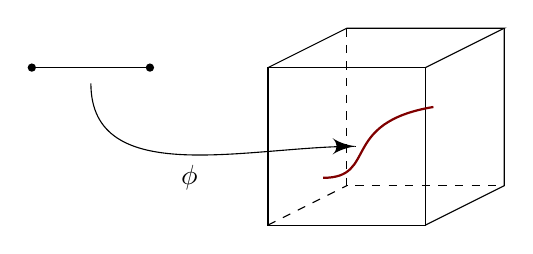
\begin{tikzpicture}
        \draw (0, 0) node [circ] {} -- (1.5, 0) node [circ] {};

        \draw (3, 0) rectangle (5, -2);
        \draw (3, 0) -- (4, 0.5) -- (6, 0.5) -- (5, 0);
        \draw (6, 0.5) -- (6, -1.5) -- (5, -2);
        \draw [dashed] (4, 0.5) -- (4, -1.5) -- (6, -1.5);
        \draw [dashed] (3, -2) -- (4, -1.5);

        \draw (0.75, -0.2) edge [out=270, in=180] (4.1, -1);

        \node at (2, -1.4) {$\phi$};

        \draw [->] (4.099, -1) -- (4.1, -1);

        \draw [thick, mred](3.7, -1.4) .. controls (4.4, -1.4) and (3.9, -0.7) .. (5.1, -0.5);
      \end{tikzpicture}
    \end{center}
    In string theory, we often have fields $\phi: \Sigma \to N$, where $N$ is a \emph{Calabi-Yau manifold}.

    In pion physics, $\pi(x)$ describes a map $\phi: (\R^4, \eta) \to G/H$, where $G$ and $H$ are Lie groups.

    Of course, we can go beyond scalar fields. We can also have fields with non-zero spin such as fermions or gauge fields, eg. a connection on a principal $G$-bundle, as we will figure out later. These are fields that carry a non-trivial representation of the Lorentz group. There is a whole load of things we can choose for our field.

    Whatever field we choose, we let $\mathcal{C}$\index{$\mathcal{C}$} be the space of all field configurations, ie. a point $\phi \in \mathcal{C}$ represents a picture of our field across all of $M$. Thus $\mathcal{C}$ is some form of function space and will typically be infinite dimensional. This infinite-dimensionality is what makes QFT hard, and also what makes it interesting.

  \item We choose an action. An \emph{action} is just a function $S: \mathcal{C} \to \R$. You tell me what the field looks like, and I will give you a number, the value of the action. We often choose our action to be local, in the sense that we assume there exists some function $\mathcal{L}(\phi, \partial \phi, \cdots)$ such that
    \[
      S[\phi] \int_M\d^4 x \sqrt{g}\; \mathcal{L}(\phi(x), \partial\phi (x)).
    \]
    The physics motivation behind this choice is obvious --- we don't want what is happening over here to depend on what is happening at the far side of Pluto. However, this assumption is actually rather suspicious, and we will revisit this later.

    For example, we have certainly met actions that look like
    \[
      S[\phi] = \int \d^4 x\; \left(\frac{1}{2} (\partial \phi)^2 + \frac{m^2}{2} \phi^2 + \frac{\lambda}{4!} \phi^4\right),
    \]
    and for gauge fields we might have seen
    \[
      S[A] = \frac{1}{4} \int \d^4 x\; F_{\mu\nu}F^{\mu\nu}.
    \]
    If we have a coupled fermion field, we might have
    \[
      S[A, \psi] = \frac{1}{4} \int \d^4 x\; F_{\mu\nu}F^{\mu\nu} + \bar\psi (\slashed{D} + m) \psi.
    \]
    But recall when we first encountered Lagrangians in classical dynamics, we worked with \emph{lots} of different Lagrangians. We can do whatever thing we like, make the particle roll down the hill and jump into space etc, and we get to deal with a whole family of different Lagrangians. But when we come to quantum field theory, the choices seem to be rather restrictive. Why can't we choose something like
    \[
      S[A] = \int F^2 + F^4 + \cosh(F^2) + \cdots?
    \]
    It turns out we can, and in fact we \emph{must}. We will have to work with something much more complicated.

    But then what were we doing in the QFT course? Did we just waste time coming up with tools that just work with these very specific examples? It turns out not. We will see that there are very good reasons to study these specific actions.
  \item What do we compute? In this course, the main object we'll study is the \term{partition function}
    \[
      \mathcal{Z} = \int_\mathcal{C} \D \phi\; e^{-S[\phi]/\hbar},
    \]
    which is some sort of integral over the space of all fields. Note that the minus sign in the exponential is for the Euclidean signature. If we are not Euclidean, we get some $i$'s instead.

    We will see that the factor of $e^{-S[\phi]/\hbar}$ means that as $\hbar \to 0$, the dominant contribution to the partition function comes from stationary points of $S[\phi]$ over $\mathcal{C}$, and this starts to bring us back to the classical theory of fields. The effect of $e^{-S[\phi]/\hbar}$ is to try to suppress ``wild'' contributions to $\mathcal{Z}$, eg. where $\phi$ is varying very rapidly or $\phi$ takes very large values.

     Heuristically, just as in statistical physics, we have a competition between the two factors $\D \phi$ and $e^{-S[\phi]/\hbar}$. The action part tries to suppress crazy things, but how well this happens depends on how much crazy things are happening, which is measured by the measure $\D \phi$. We can think of this $\D \phi$ as ``entropy''. However, the problem is, the measure $\D \phi$ on $\mathcal{C}$ doesn't actually exist!

    Understanding what we mean by this path integral, and what this measure actually is, and how we can actually compute this thing, and how this has got to do with the canonical quantization operators we had previously, is the main focus of the first part of this course.
\end{enumerate}

\section{QFT in zero dimensions}
We start from the simplest case we can think of, namely quantum field theory in zero dimensions. You might think this is rather trivial, and it is. And this is good.

In $d = 0$, if our universe $M$ is connected, then the only choice of $M$ is $\{\mathrm{pt}\}$. There is a no possibility for a field to have spin, because the Lorentz group is trivial. Our fields are scalar, and the simplest choice is just a single field $\phi: \{\mathrm{pt}\} \to \R$, ie. just a real variable. Similarly, we simply have $\mathcal{C} \cong \R$. This is \emph{not} an infinite-dimensional space.

The action is just a normal function $S: \mathcal{C} \cong \R \to \R$ of one real variable. The path integral measure $\D \phi$ can be taken to just be the standard (Lebesgue) measure $\d \phi$ on $\R$. So our partition function is just
\[
  \mathcal{Z} = \int_\R \d \phi\; e^{-S(\phi)/\hbar},
\]
where we assume $S$ is chosen so that this converges. This happens if $S$ grows sufficiently large as $\phi \to \pm \infty$.

More generally, we may wish to compute \term{correlation functions}, ie. we pick another function $f(\phi)$ and compute the \term{expectation}\index{$\bra f(\phi)\ket$}
\[
  \bra f(\phi)\ket = \frac{1}{\mathcal{Z}} \int \d \phi\; f(\phi) e^{-S(\phi)/\hbar}.
\]
Again, we can pick whatever $f$ we like as long as the integral converges. In this case, $\frac{1}{\mathcal{Z}} e^{-S(\phi)/\hbar}$ is a probability distribution on $\R$, and as the name suggests, $\bra f(\phi)\ket$ is just the expectation value of $f$ in this distribution. Later on, when we study quantum field theory in higher dimensions, we can define more complicated $f$ by evaluating $\phi$ at different points, and we can use this to figure out how the field at different points relate to each other.

Our action is taken to have a series expansion in $\phi$, so in particular we can write
\[
  S(\phi) = \frac{m^2 \phi^2}{2} + \sum_{n = 3}^N g_n \frac{\phi^n}{n!}.
\]
We didn't put in a constant term, as it would just give us a constant factor in $\mathcal{Z}$. We could have included linear terms, but we shall not. The important thing is that $N$ has to be even, so that the asymptotic behaviour of $S$ is symmetric in both sides.

Now the partition function is a function of all these terms: $\mathcal{Z} = \mathcal{Z}(m^2, g_n)$. Similarly, $\bra f\ket$ is again a function of $m^2$ and $g_n$, and possibly other things used to define $f$ itself.

Note that \emph{nothing} depends on the field, because we are integrating over all possible fields.

\subsection{Free theories}
We consider the simplest possible QFT. These QFT's are free, and so $S(\phi)$ is at most quadratic. Classically, this implies the equations of motions are linear, and so there is superposition, and thus the particles do not interact.

Let $\phi: \{\mathrm{pt}\} \to \R^n$ be a field with coordinates $\phi^a$, and define
\[
  S(\phi) = \frac{1}{2} M(\phi, \phi) = \frac{1}{2} M_{ab} \phi^a \phi^b,
\]
where $M: \R^n \times \R^n \to \R$ is a positive-definite symmetric matrix. Then the partition function $\mathcal{Z}(M)$ is just a Gaussian integral:
\[
  \mathcal{Z}(M) = \int_{\R^n} \d^n \phi\; e^{- \frac{1}{2\hbar} M(\phi, \phi)} = \frac{(2 \pi \hbar)^{n/2}}{\sqrt{\det{M}}}.
\]
Indeed, since $M$ is symmetric, there exists an orthogonal transformation $O: \R^n \to \R^n$ that diagonalizes it. The measure $\d^n \phi$ is invariant under orthogonal transformations. So in terms of the eigenvectors of $M$, this just reduces to a product of $n$ 1D Gaussian integrals of this type, and this is a standard integral:
\[
  \int \d \chi e^{-m\chi^2/2\hbar} = \sqrt{\frac{2\pi \hbar}{m}}.
\]
In our case, $m > 0$ runs over all eigenvalues of $M$.

A small generalization is useful. We let
\[
  S(\phi) = \frac{1}{2} M(\phi, \phi) + J(\phi),
\]
where $J: \R^n \to \R$ is some linear map (we can think of $J$ as a (co)vector, and also write $J(\phi) = J \cdot \phi$). $J$ is a \emph{source} in the classical case. Then in this theory, we have
\[
  \mathcal{Z}(M, J) = \int_{\R^n} \d^n \phi\; \exp\left(-\frac{1}{\hbar}\left(\frac{1}{2} M(\phi, \phi) + J(\phi)\right)\right).
\]
We now let $\tilde{\phi} = \phi + M^{-1}J$. In other words,
\[
  \tilde{\phi}^a = \phi^a + (M^{-1})^{ab} J_b.
\]
The inverse exists because $M$ is assumed to be positive definite. We can now complete the square to find
\begin{align*}
  \mathcal{Z}(M, J) &= \int_{\R^n} \d^n \tilde{\phi} \;\exp\left(\frac{-1}{2\hbar}M(\tilde{\phi}, \tilde{\phi}) + \frac{1}{2\hbar}M^{-1}(J, J)\right)\\
  &= \exp\left(\frac{1}{2\hbar}M^{-1}(J, J)\right)\int_{\R^n} \d^n \tilde{\phi} \;\exp\left(\frac{-1}{2\hbar}M(\tilde{\phi}, \tilde{\phi})\right)\\
  &= \exp\left(\frac{1}{2\hbar}M^{-1}(J, J)\right) \frac{(2\pi \hbar)^{n/2}}{\sqrt{\det M}}.
\end{align*}
This generalization is useful because it allows us to compute correlation functions.

Consider the case without a source, and let $P: \R^n \to \R$ be a polynomial. We look at
\[
  \bra P(\phi)\ket = \frac{1}{\mathcal{Z}(M)} \int_{\R^n} \d^n \phi\; P(\phi) \exp\left(-\frac{1}{2\hbar} M(\phi, \phi)\right).
\]
By linearity, it suffices to consider the case where $P$ is just a monomial, so
\[
  P(\phi) = \prod_{i = 1}^m (\ell_i(\phi)),
\]
for $\ell_i : \R^n \to \R$ linear maps. Now if $m$ is odd, then clearly $\bra P(\phi)\ket = 0$, since this is an integral of an odd function. When $m = 2k$, then we have
\[
  \bra P(\phi) \ket = \frac{1}{\mathcal{Z}(M)} \int \d^n \phi\; (\ell_i\cdot \phi) \cdots (\ell_{2k} \cdot \phi) \exp\left(-\frac{1}{2\hbar}M (\phi, \phi) - \frac{J \cdot \phi}{\hbar}\right).
\]
Here we are eventually going to set $J = 0$, but for the time being, we will be silly and put the source there. The relevance is that we can then think of our factors $\ell_i \cdot \phi$ as derivatives with respect to $J$:
\begin{align*}
  \bra P(\phi)\ket &= \frac{(-\hbar)^{2k}}{\mathcal{Z}(M)} \int \d^n \phi \; \prod_{i = 1}^{2k} \left(\ell_i \cdot \frac{\partial}{\partial J}\right) \exp\left(-\frac{1}{2\hbar} M(\phi, \phi) - \frac{J\cdot \phi}{\hbar}\right)\\
  \intertext{Since the integral is absolutely convergent, we can move the derivative out of the integral, and get}
  &= \frac{(-\hbar)^{2k}}{\mathcal{Z}(M)} \prod_{i = 1}^{2k} \left(\ell_i \cdot \frac{\partial}{\partial J}\right) \int \d^n \phi \; \exp\left(-\frac{1}{2\hbar} M(\phi, \phi) - \frac{J\cdot \phi}{\hbar}\right)\\
  &= \hbar^{2k} \prod_{i = 1}^{2k} \left(\ell_i \cdot \frac{\partial}{\partial J}\right) \exp\left(\frac{1}{2\hbar}M^{-1}(J, J)\right).
\end{align*}
When each derivative $\ell \cdot \frac{\partial}{\partial J}$ acts on the exponential, we obtain a factor of
\[
  \frac{1}{\hbar} M^{-1}(J, \ell).
\]
in front. At the end, we are going to set $J = 0$. So we only get contributions if and only if exactly half (ie. $k$) of the derivatives act on the exponential, and the other $k$ act on the factor in front.

We let $\sigma$ denote a (complete) pairing of the set $\{1, \cdots, 2k\}$, and $\Pi_{2k}$ be the set of all such pairings. For example, if we have $k = 2$, then the possible pairings are $\{(1, 2), (3, 4)\}$, $\{(1, 3), (2, 4)\}$ and $\{(1, 4), (2, 3)\}$:
\begin{center}
  \begin{tikzpicture}
    \node [circ] at (0, 0) {};
    \node [circ] at (1, 0) {};
    \node [circ] at (1, 1) {};
    \node [circ] at (0, 1) {};
    \draw (0, 0) -- (0, 1);
    \draw (1, 0) -- (1, 1);

    \begin{scope}[shift={(3, 0)}]
      \node [circ] at (0, 0) {};
      \node [circ] at (1, 0) {};
      \node [circ] at (1, 1) {};
      \node [circ] at (0, 1) {};
      \draw (0, 0) -- (1, 0);
      \draw (0, 1) -- (1, 1);
    \end{scope}

    \begin{scope}[shift={(6, 0)}]
      \node [circ] at (0, 0) {};
      \node [circ] at (1, 0) {};
      \node [circ] at (1, 1) {};
      \node [circ] at (0, 1) {};
      \draw (0, 0) -- (1, 1);
      \draw (1, 0) -- (0, 1);
    \end{scope}
  \end{tikzpicture}
\end{center}
In general, we have
\[
  |\Pi_{2k}| = \frac{(2k)!}{2^k k!},
\]
and we have
\begin{thm}[Wick's theorem]\index{Wick's theorem}
  For a polynomial
  \[
    P(\phi) = \prod_{i = 1}^{2k} \ell_i(\phi),
  \]
  we have
  \[
    \bra P(\phi)\ket = \hbar^{2k}\sum_{\sigma \in \Pi_{2k}} \prod_{i \in \{1, \cdots, 2k\}/\sigma} M(\ell_i, \ell_{\sigma(i)}).
  \]
  where the $\{1, \cdots, 2k\}/\sigma$ says we sum over each pair $\{i, \sigma(i)\}$ only once, rather than once for $(i, \sigma(i))$ and another for $(\sigma(i), i)$.
\end{thm}
This is in fact the version of Wick's theorem for this 0d QFT, and $M^{-1}$ plays the role of the propagator.

For example, we have
\[
  \bra \ell_1(\phi), \ell_2(\phi)\ket = \hbar M^{-1} (\ell_1, \ell_2).
\]
We can represent this by the diagram
\begin{center}
  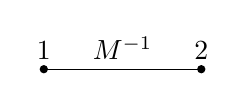
\begin{tikzpicture}
    \node [circ] at (0, 0) {};
    \node [circ] at (2, 0) {};

    \node [above] at (0, 0) {$1$};
    \node [above] at (2, 0) {$2$};
    \draw (0, 0) -- (2, 0) node [pos=0.5, above] {$M^{-1}$};
  \end{tikzpicture}
\end{center}
Similarly, we have
\begin{multline*}
  \bra \ell_1(\phi) \cdots \ell_4(\phi)\ket = \hbar^2 \Big(M^{-1}(\ell_1, \ell_2) M^{-1}(\ell_3, \ell_4) \\
  + M^{-1}(\ell_1, \ell_3) M^{-1}(\ell_2, \ell_4) + M^{-1}(\ell_1, \ell_4) M^{-1}(\ell_2, \ell_3)\Big).
\end{multline*}
This is purely combinatorial.

This is about all we can say for free 0d QFTs. There is an analogue for ``fermions'', which is put in the first example sheet.

\subsection{Interacting theories}
Physically interesting theories contain interactions, ie. $S(\phi)$ is non-quadratic. Typically, if we are trying to compute
\[
  \int \d^n \phi P(\phi) \exp\left(-\frac{S(\phi)}{\hbar}\right),
\]
these things involve transcendental functions and, except in very special circumstances, is just too hard. We usually cannot perform these integrals analytically.

In perturbation theory, we use the fact that
\[
  \mathcal{Z} = \int \d^n \phi\; \exp\left(-\frac{S(\phi)}{\hbar}\right)
\]
has an \term{asymptotic series} as $\hbar \to 0^+$. Recall that a series
\[
  \sum_{n = 0}^\infty f_n(\hbar)
\]
is an \emph{asymptotic series} for $\mathcal{Z}(\hbar)$ if for any fixed $N \in \N$, if we write $\mathcal{Z}_N(\hbar)$ for the first $N$ terms on the RHS, then
\[
  \lim_{\hbar \to 0^+} \frac{|\mathcal{Z}(\hbar) - \mathcal{Z}_N(\hbar)|}{\hbar^N} \to 0.
\]
Thus as $\hbar \to 0^+$, we get an arbitrarily good approximation to what we really wanted from any finite number of terms. But the series will in general diverge if try to fix $\hbar \in \R_{> 0}$, and include increasingly many terms.

Most of the expansions we do in quantum field theories are of this nature.

In our case, note that the integral very likely diverges if $\hbar < 0$, as usually $S(\phi) \to \infty$ as $\phi \to \pm\infty$. So it can't have a Taylor series expansion around $\hbar = 0$, as such expansions have to be valid in a disk in the complex plane. The best we can hope for is an asymptotic series.

Suppose $S(\phi)$ is smooth with a global minimum at $\phi = \phi_0 \in \R^n$, where the Hessian
\[
  \left.\frac{\partial^2 S}{\partial \phi^a \partial \phi^b}\right|_{\phi_0}
\]
is positive definite. Then by Laplace's method/Watson's lemma, we have an asymptotic series
\[
  \mathcal{Z}(\hbar) \sim (2\pi \hbar)^{n/2} \frac{\exp\left(-\frac{S(\phi_0)}{\hbar}\right)}{\sqrt{\det \partial_a \partial_b S(\phi_0)}} \left(1 + A \hbar + B \hbar^2 + \cdots\right).
\]
We will not prove this, but the proof is available in any standard asymptotic methods textbook. The leading term involves the action evaluated on the classical solution $\phi_0$, and is known as the \term{semiclassical term}. Every thing we did last term with tree diagrams was about calculating the first term. The remaining terms are called the \term{quantum correction}.

We recall the definition of an asymptotic series. Let
\begin{eg}
  Let's consider a single scalar field $\phi$ with action
  \[
    S(\phi) = \frac{m^2}{2}\phi^2 + \frac{\lambda}{4!} \phi^4,
  \]
  where $m^2, \lambda > 0$. The action has a unique global minimum at $\phi_0 = 0$. The action evaluated at $\phi_0 = 0$ vanishes, and $\partial^2 S/\hbar = m^2$. So the leading term in the asymptotic expansion of $\mathcal{Z}(\hbar, m \lambda)$ is
  \[
    \frac{(2\pi \hbar)^{1/2}}{m}.
  \]
  Further,
  \begin{align*}
    \mathcal{Z}(\hbar, m, \lambda) &= \int_\R \d \phi \; \exp\left(\frac{-1}{\hbar}\left(\frac{m^2}{2} \phi^2 + \frac{\lambda}{4!}\phi^4\right)\right)\\
    &= \frac{\sqrt{2\hbar}}{m} \int \d \tilde{\phi} \exp\left(-\tilde{\phi}^2 \right) \exp\left( - \frac{\lambda \hbar^4}{4! m^4} \tilde{\phi}^4\right)\\
    &\sim \frac{\sqrt{2\hbar}}{m} \sum_{n = 0}^N \left(\frac{-\lambda \hbar^4}{m^4 4!}\right)^n \frac{1}{n!} \int \d \tilde{\phi}\;e^{- \tilde{\phi}^2}\tilde{\phi}^{4n}\\
    &= \frac{\sqrt{2\hbar}}{m} \sum_{n = 0}^N \left(\frac{-\lambda \hbar^4}{m^4 4!}\right)^n \frac{1}{n!} \Gamma\left(2n + \frac{1}{2}\right).
  \end{align*}
  We will get to understand these numbers much more in terms of Feynman diagrams later. % check!
\end{eg}

\printindex
\end{document}
